\documentclass[11pt,a4paper]{article}
\usepackage[margin=25mm]{geometry}
\usepackage[T1]{fontenc}
\usepackage{lmodern,microtype,amsmath,amssymb,booktabs,longtable,array,graphicx}
\usepackage{xcolor,listings,enumitem,caption,tikz}
\usetikzlibrary{arrows.meta,positioning,fit}
\usepackage[hidelinks,breaklinks]{hyperref}
\usepackage{xurl}
\definecolor{ink}{HTML}{20384B}
\definecolor{light}{HTML}{F1F4F6}
\lstset{basicstyle=\ttfamily\footnotesize,breaklines=true,columns=fullflexible,keepspaces=true,showstringspaces=false,backgroundcolor=\color{light},frame=single,rulecolor=\color{light},xleftmargin=5pt,xrightmargin=5pt,aboveskip=10pt,belowskip=10pt}
\setlist{itemsep=3pt,topsep=5pt}
\setlength{\emergencystretch}{3em}
\newcommand{\code}[1]{\nolinkurl{#1}}
\hypersetup{pdftitle={Reproducible ensemble data assimilation with ICESEE},pdfauthor={Brian Kyanjo}}
\newcommand{\Ne}{N_{\mathrm e}}
\newcommand{\revision}{3748e416d3a8120cc860119bd7224c6f9ad41ff7}
\title{Reproducible ensemble data assimilation with ICESEE\\Distributed execution, recoverable histories and a production operations protocol}
\author{Brian Kyanjo}
\date{Technical report and preprint draft\\10 November 2026}
\begin{document}
\maketitle
\begin{abstract}
Ensemble data assimilation requires a reliable relationship between the mathematical update, the ownership of model state, the time associated with observations, and the files used to resume and interpret a calculation. We describe developments in the Ice Sheet State and Parameter Estimator (ICESEE) that make these relationships explicit. The implementation separates replicated and distributed state, supports file-backed ensemble analysis and native distributed model contexts, streams observation products and state rows through an ensemble-space transform, and records checkpoint and history metadata. A shared state-column contract aligns initialization, forecasts, observations and process noise, and refuses incompatible old output. We provide the implemented transform rather than identifying it with a textbook Kalman gain without qualification. Existing verification records include a five-year, 32-member Icepack experiment in three execution modes, a restart experiment crossing analysis events, and continuous integration with real MPI tests. All three five-year simulations exited successfully; the simulation allocation and a subsequent verification-only allocation timed out during output verification, whose remaining checks subsequently passed in a bounded read-only scan. These are operational and numerical-integrity results, not a controlled scaling study or an independent assessment of physical accuracy. A detailed operations protocol, source map and reproducibility requirements make the report usable for student-led production work and identify the evidence still needed for a journal submission.
\end{abstract}
\noindent\textbf{Code basis.} ICESEE \code{features_debug}, commit \code{3748e416d3a8120cc860119bd7224c6f9ad41ff7}. The literal hash is printed in the provenance table below. This report identifies a development snapshot; it does not assign a new software release number.\par
\vspace{5pt}
\noindent\textbf{Reading route.} Sections 2--6 explain the numerical and computational contracts. Sections 7--9 give the evidence and its limits. Sections 10--12 and the appendices provide an operating manual. The companion repository handbook supplies command-level references.
\newpage
\setcounter{tocdepth}{1}
\tableofcontents
\newpage

\section{Purpose and relationship to the earlier ICESEE paper}
ICESEE combines ensemble data assimilation with model-specific forecast and inversion routines. Its original model-description paper introduced the library, ensemble filtering, coupling to ice-sheet models, and illustrative scientific and performance experiments \cite{kyanjo2026}. The present report concerns a later engineering and reproducibility layer: what constitutes a state, where it is owned, which time it represents, how bounded analysis is performed, how a closed output history is reconstructed, and what evidence an operator must retain.

The distinction matters for a long-running research code. A mathematically plausible analysis can still be attached to the wrong model time. A successful forecast step does not establish that an ensemble history was fully written. A file-backed algorithm can avoid a full ensemble allocation during analysis while retaining a full-member temporary elsewhere. A mode that runs one adapter does not establish the same capabilities for another adapter. These are testable contracts, and each needs a separate statement.

We organize the contribution around five implemented developments: explicit state ownership; bounded ensemble-space analysis and native model contexts; checkpoint and history recovery; a common state-column clock; and provenance-aware verification and operations. We do not claim that grouped local analysis, covariance localization, or observation-error modes are first introduced here. The August 2026 public replies associated with the earlier manuscript already discuss those topics \cite{egusphere2026}. Here they are explained only as necessary to specify the current implementation.

The report has two audiences. Students need concrete rules for choosing an environment, running an experiment, identifying a failure, and handing work to another operator. Developers need the ownership, communication and numerical invariants that must survive a code change. Neither audience benefits from an unqualified assertion that a branch is ``production ready.'' Instead, we state the exact verified configurations and the checks required for a new one.

\section{Source identity and the computational experiment}
\subsection{A source revision is part of the experiment}
The code basis is the published development branch at the hash shown in Table~\ref{tab:source}. At the time of inspection, \code{main} and \code{features_debug} differed. A fresh clone of the default branch therefore cannot be assumed to contain the implementation described here. Pull request 72 remained open in the retained publication record. Documentation work does not merge that pull request or update an installation's parent repository pin.

\begin{table}[htbp]\centering\small
\caption{Source identities inspected for this report. Long hashes, rather than moving branch names, identify the snapshots.}\label{tab:source}
\begin{tabular}{p{.25\linewidth}p{.68\linewidth}}\toprule
Component & Inspected identity\\\midrule
ICESEE development source & \code{3748e416d3a8120cc860119bd7224c6f9ad41ff7}\\
ICESEE default branch & \code{3d7e6e757e07b80dcca1fdd65dffb8ca8853316a}\\
ICESEE-Spack main & \code{68e37fffcd13cc60636028d051d4637e7f573d4f}\\
ICESEE-Containers main & \code{884cc3046a26b5999f6db16a98ad38a96bfdbcfd}\\
Wiki before this documentation update & \code{79a45cc643f2a2943e10e8d8d1dccf99253be69e}\\\bottomrule
\end{tabular}
\end{table}

The repository's metadata are not internally consistent at this snapshot: \code{pyproject.toml} declares version 0.1.9 and an MIT license string; \code{CITATION.cff} declares 1.0.0; the top-level license text is BSD 2-Clause. The original paper and the citation file also refer to different archive identifiers. The report therefore uses a commit identity, cites the existing paper as prior work, and does not represent an older archive as containing these developments. Resolving release metadata and depositing the exact new source and data are required before submission.

The execution environment is equally important. A source checkout, a Python editable installation, a Spack environment and a container image are distinct objects. The interpreter can import an older source path even after a newer checkout is fetched. Before running, record the executable, \code{ICESEE.__file__}, the package root, the Git hash, local changes, the MPI library reported by \code{mpi4py}, and HDF5 parallel support. These records must be generated within the actual batch environment.

\subsection{What must accompany a result}
An experiment consists of source, configuration, inputs, numerical environment, launch topology, random policy, output and validation. Save the resolved configuration as well as the original YAML and CLI arguments. Preserve input checksums or persistent dataset identifiers. Record the number of world ranks, ranks in each model group, thread limits and node placement. Save simulation exit status separately from the status of a postprocessing or verification command.

A branch name alone is insufficient because it can move; a container tag alone is insufficient for the same reason. A YAML file alone is insufficient because command-line options can replace its values. A final image is insufficient because it can hide missing members or an incorrect observation schedule. These records are small relative to the ensemble history and allow another operator to reconstruct the intended calculation.

\section{The numerical contract}
\subsection{State and observation notation}
Let \(n\) be the number of packed state entries, \(m\) the active observation count and \(\Ne\) the ensemble size. We arrange members in columns,
\begin{equation}
 X^f=[x_1^f,\ldots,x_{\Ne}^f]\in\mathbb R^{n\times\Ne},\qquad
 A=X^f-\bar x^f\mathbf1^T.
\end{equation}
For a potentially nonlinear observation operator \(h\), evaluate each forecast member first:
\begin{equation}
 Y=[h(x_1^f),\ldots,h(x_{\Ne}^f)],\quad
 \bar y^f=Y\mathbf1/\Ne,\quad Y'=Y-\bar y^f\mathbf1^T.
\end{equation}
In particular, \(h(A)\) is not a replacement for \(Y'\) when \(h\) is nonlinear. The observation vector \(y\) has length \(m\). The conventional stochastic analysis provides the familiar reference expression
\begin{equation}
 X^a=X^f+AY'^T\{Y'Y'^T+(\Ne-1)R\}^{-1}D,
 \qquad D=y\mathbf1^T+E-Y,
 \label{eq:textbook}
\end{equation}
with suitable assumptions on errors and the inverse \cite{evensen2003,burgers1998}. This equation establishes dimensions and terminology. The implemented factor formulation below must be stated separately.

\subsection{The implemented factor and ensemble transform}
\code{StochasticAnalysisProducts.add_chunk} in \code{src/parallelization/distributed_analysis.py} forms a factor \(F=Y'+E\). For \code{stochastic_R} and \code{generated_R}, an explicit error array \(E\), aligned with the forecast observation rows and members, is required. The innovations are \(D=y\mathbf1^T+E-Y\). For \code{legacy_prior_anomalies}, the implementation instead sets \(E=Y'\) and \(D=y\mathbf1^T-Y\). These policies are not interchangeable descriptions of an identical experiment.

For observation chunks indexed by \(b\), accumulate
\begin{equation}
 C=\sum_b Y_b'^TF_b,\qquad
 G=\sum_b F_b^TF_b,\qquad
 B=\sum_b F_b^TD_b.
 \label{eq:products}
\end{equation}
Each product has shape \(\Ne\times\Ne\). After reduction over distinct observation owners, \code{ensemble_transform_from_products} symmetrizes \(G\), computes its eigendecomposition, orders eigenvalues from largest to smallest, clips negative values to zero, and retains enough eigenvalues to reach a default fraction 0.999 of their sum. An additional machine-precision threshold excludes numerically negligible retained values. With the resulting truncated pseudoinverse \(G_q^+\), the returned transform is
\begin{equation}
 T=I+C G_q^+G_q^+B,\qquad X^a=X^f T.
 \label{eq:transform}
\end{equation}
Both pseudoinverse factors in this equation are intentional: they are present in the source. An explanation with only one factor would describe a different computation.

To interpret the products, for an untruncated singular value decomposition \(F=U\Sigma V^T\),
\begin{equation}
 (FF^T)^+=F(F^TF)^+(F^TF)^+F^T.
\end{equation}
Consequently the product form represents \(Y'^T(FF^T)^+D\) without an observation-by-observation matrix. With truncation, the corresponding retained singular subspace must be used consistently. Since \(\mathbf1^TY'^T=0\), \(\mathbf1^T(T-I)=0\) in exact arithmetic, so applying the increment through raw members or anomalies is consistent in that algebraic sense.

This factor form does not by itself prove equality to Eq.~\ref{eq:textbook} for an arbitrary supplied \(R\). In a finite sample,
\begin{equation}
 FF^T=Y'Y'^T+EE^T+Y'E^T+EY'^T.
\end{equation}
The cross terms do not vanish merely because two random variables are independent in expectation. The retained spectrum, error generator, centering and scaling are all part of the numerical method. Scientific comparisons must retain these choices and test the desired relation empirically or analytically. The present developments preserve the selected implementation while changing ownership and storage.

\subsection{Inflation, localization and physical postprocessing}
An ensemble-space representation avoids explicit allocation of the state covariance \(AA^T/(\Ne-1)\). It does not remove finite-ensemble sampling error or justify ignoring localization. The code includes global and grouped local analysis paths. A grouped local request describes target state rows, observation coordinates, observation kinds and permitted couplings. All accepted observation kinds for one target enter the same assembled local transform; treating each kind as a separate sequential filter can change the result.

Inflation changes spread and therefore belongs to the experiment, even when it is applied in a bounded row loop. Record its configured value and the selected analysis path. The default PIG file inspected here specifies 1.15; that is an example value, not a recommendation for every model. Localization length scales and support rules require a scientific justification for each observation network.

After analysis, the model adapter restores physical consistency. Geometry, surface, thickness, diagnostic velocities and inferred parameters cannot be treated as unrelated vector entries merely because they are packed together. Native fields must be updated and halo values refreshed before subsequent model solves. A post-analysis projection can also alter a nominal Kalman increment. Record the projection policy and test the constraints it is meant to enforce.

The shared mode-1/mode-2 control helper first relaxes increments, optionally caps them by variable, inflates anomalies about the controlled row mean, restores frozen variables and applies the bed-update gate. Model geometry and inference callbacks follow in their configured paths. These operations can change the posterior. The streamed spectral-energy setting is not a universal switch: some direct/local paths retain a hard-coded 0.999 threshold. Verify the active implementation before treating a control change as equivalent across modes.

The code detects ensembles whose observed-space anomalies are negligible compared with the forecast magnitude. In the distributed product implementation the default relative threshold is \(10^{-8}\). Refusing that analysis prevents division by round-off directions. Increasing numerical tolerances or introducing an unreviewed perturbation solely to pass this guard changes the experiment. Diagnose the initial ensemble and the configured process-noise schedule instead.

\section{State ownership and process topology}
\subsection{Replicated and distributed state are different contracts}
A model can return a complete member on every rank in its model communicator, or disjoint owned pieces of that member. \code{src/utils/state_ownership.py} makes this difference explicit. For replicated state, the global member dimension equals one local dimension; concatenating ranks duplicates the state. For distributed state, the global dimension is the sum of disjoint owned dimensions. Array shape is not enough to determine which contract holds.

The small Lorenz example is replicated. Its directory and function names say \code{lorenz96}, but its right-hand side is the three-variable system
\begin{align}
 \dot x&=\sigma(y-x),&\dot y&=x(\rho-z)-y,&\dot z&=xy-\beta z.
\end{align}
These are Lorenz-63 equations. We retain existing path names for executable compatibility and identify the actual equations in the scientific description. Its integration tests establish properties of this small implementation, not of a high-dimensional Lorenz-96 system.

In finite-element models, a local vector can include owned entries and ghosts. Only owned entries belong in a global state partition. Ghost entries support stencil or finite-element communication and must not be counted a second time. A segmented state layout describes each named variable separately, preserving variable-major packing while concatenating only the locally owned pieces. The partition validator must detect gaps and overlaps for every variable.

\subsection{Two levels of parallel work}
Native distributed execution separates model groups from the ensemble communicator. A spatial communicator joins ranks that cooperate on one member's forecast. An ensemble communicator joins corresponding spatial positions across groups and assembles the same state rows for different members. More members than groups can be scheduled in rounds. Thus \(P=\Ne P_s\) is not a general requirement; the topology must permit a group to handle several members.

\begin{figure}[htbp]\centering
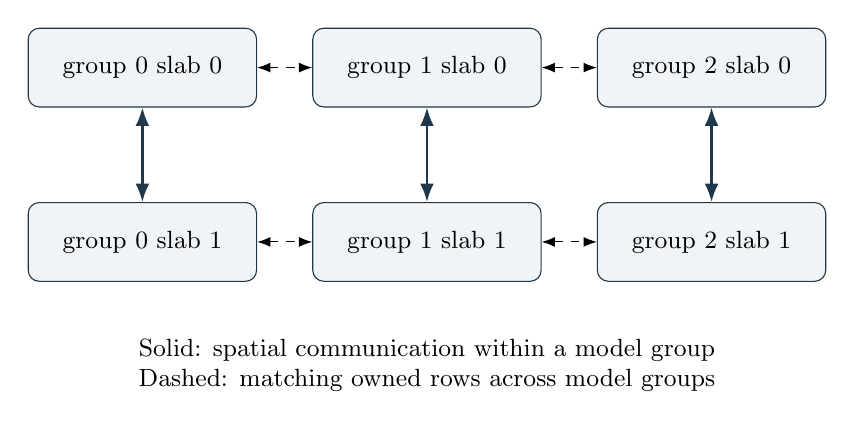
\begin{tikzpicture}[>=Latex,every node/.style={font=\small},box/.style={draw=ink,rounded corners,minimum width=29mm,minimum height=10mm,fill=light}]
\node[box](a){group 0 slab 0};\node[box,right=7mm of a](b){group 1 slab 0};\node[box,right=7mm of b](c){group 2 slab 0};
\node[box,below=12mm of a](d){group 0 slab 1};\node[box,right=7mm of d](e){group 1 slab 1};\node[box,right=7mm of e](f){group 2 slab 1};
\draw[<->,thick,ink](a)--(d);\draw[<->,thick,ink](b)--(e);\draw[<->,thick,ink](c)--(f);
\draw[<->,dashed](a)--(b);\draw[<->,dashed](b)--(c);\draw[<->,dashed](d)--(e);\draw[<->,dashed](e)--(f);
\node[below=6mm of e,align=center]{Solid: spatial communication within a model group\\Dashed: matching owned rows across model groups};
\end{tikzpicture}
\caption{Conceptual native process grid. Group identity is distinct from member identity; groups may advance multiple stable member IDs. This sketch is not an assertion that every adapter uses the same placement.}\label{fig:topology}
\end{figure}

Node locality is an operational property, not a consequence of a mode number. PIG supports node-local native model groups, and a retained topology check confirmed locality for the five-year experiment. MPI launch order, scheduler rank placement and the ranks-per-model value must all agree. Avoid assuming an arithmetic rank split automatically preserves locality on a multi-node allocation.

Every collective operation has a participant set. A collective HDF5 open on a model communicator requires all ranks in that communicator to participate. A model-group-root-only write cannot safely trigger a world- or shared-communicator collective. Earlier repairs separated collective window preparation from root-only writes. This rule generalizes to barriers, broadcasts, close operations and recovery: after one rank fails, arbitrary further collectives can hang.

\section{Execution modes and memory}
\subsection{What a mode selects}
Mode 0 provides the serial orchestration path. Mode 1 provides in-memory parallel ensemble work. Mode 2 uses file-backed ensemble orchestration and bounded analysis paths. Mode 3 dispatches to a registered native adapter and can retain model-native distributed fields. A mode does not select a different scientific filter by implication, and it does not guarantee that every adapter has the same restart, localization, inversion or spatial support.

The generic native application path has explicit restrictions, including unsupported restart requests and certain observation-error or multi-rank configurations. The specialized PIG runner supplies capabilities beyond that generic path. Registration for Lorenz, flowline, synthetic ice stream, PIG or ISSM is evidence that a route exists; it is not evidence that all routes have been exercised at continental scale. In particular, the small Lorenz adapter can gather a compact global ensemble for legacy output without violating its small-example purpose. Universal ``no global arrays'' claims would be incorrect.

\subsection{Bounded analysis storage}
The dense ensemble contains \(n\Ne\) values. The state covariance contains \(n^2\), and a dense observation covariance contains \(m^2\). With chunks of at most \(c\) state rows and \(r\) observation rows, Eqs.~\ref{eq:products}--\ref{eq:transform} use ensemble products of order \(\Ne^2\), state work of order \(c\Ne\) and observation work of order \(r\Ne\). The spectral solve remains of order \(\Ne^3\). These are analysis workspace terms; they exclude native solver memory, history buffers, active members, caches and storage backends.

\begin{table}[htbp]\centering\small
\caption{Memory and storage quantities that must be reported separately. Bounds describe dimensions, not measured resident memory.}\label{tab:memory}
\begin{tabular}{p{.35\linewidth}p{.54\linewidth}}\toprule
Quantity & Relevant dependence or limitation\\\midrule
State covariance if formed & \(O(n^2)\), avoided by ensemble factor analysis\\
Full ensemble in memory & \(O(n\Ne)\), not a universal property of all modes\\
Analysis products & \(O(\Ne^2)\) per product\\
State update block & \(O(c\Ne)\), configured bounded row count\\
Observation block & \(O(r\Ne)\), separate from state row bound\\
Persistent native states & Owned model fields times locally active members\\
Inactive member store & Memory or member-major HDF5 backend\\
PIG native noise bridge & Canonical leader workspace \(O(n)\), 256 MiB allocation guard\\
History on disk & \(O(n\Ne(N_t+1))\) logical values for full retention\\\bottomrule
\end{tabular}
\end{table}

Native member streaming limits active model contexts by moving inactive members to a store. Store-backed analysis is an additional option and must be selected consistently with member streaming. A memory backend and an HDF5 member-major backend have different I/O costs. Lowering active-member memory can increase file traffic; a memory claim needs measurements of both the solver and the store.

The PIG process-noise bridge uses a canonical model-group leader workspace and scatters increments to the owned rows. It avoids gathering the physical member state but still has a global-size stochastic workspace, guarded at 256 MiB. Its graph transition cache has a separate 64 MiB per-process limit. These bounded allocations are material qualifications to an otherwise distributed forecast/analysis design.

\subsection{Randomness belongs to stable identities}
An ensemble member must retain its stochastic identity when ranks or groups change. The implementation includes member- and timestep-aware random policies, and the active PIG native bridge reuses the configured forecast-noise generator. A helper with a plausible seed-related name is not proof of the active path: trace the runner to its actual call site. Preserve base seeds, member IDs, noise method, correlation parameters and the time grid.

Correcting the time at which process noise is applied can change timestep-keyed draws without changing a base seed. This is expected for a clock repair and must not be described as bitwise compatibility with old trajectories. Deterministic replay of autoregressive noise also requires the policy identity and the necessary history; loading only a field array is insufficient.

\section{The state-column time contract}
\subsection{Initialization is a state rather than a forecast}
Let \(t_0,\ldots,t_{N_t}\) denote saved model-state times. Column zero stores the physical initial state. Forecast cycle \(k\), with \(0\leq k<N_t\), advances from column \(k\) to column \(k+1\). An observation attached to state column \(j>0\) is analyzed after forecast cycle \(j-1\). In the implemented sequence, configured process noise is applied before that analysis.

\begin{figure}[htbp]\centering
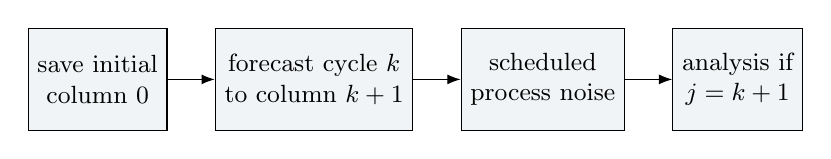
\begin{tikzpicture}[>=Latex,every node/.style={font=\small},node distance=6mm]
\node[draw,fill=light,align=center,minimum height=13mm](i){save initial\\column 0};
\node[draw,fill=light,right=of i,align=center,minimum height=13mm](f){forecast cycle \(k\)\\to column \(k+1\)};
\node[draw,fill=light,right=of f,align=center,minimum height=13mm](q){scheduled\\process noise};
\node[draw,fill=light,right=of q,align=center,minimum height=13mm](a){analysis if\\\(j=k+1\)};
\draw[->](i)--(f);\draw[->](f)--(q);\draw[->](q)--(a);
\end{tikzpicture}
\caption{The corrected clock. No extra forecast is hidden in initialization. The output contains \(N_t+1\) states for \(N_t\) forecast cycles.}\label{fig:clock}
\end{figure}

For the five-year validation, \(\Delta t=0.05\) years gives 100 cycles and 101 saved state columns. Observations at years 2, 3 and 4 correspond to columns 40, 60 and 80, and are applied after cycles 39, 59 and 79. The one-year short validation also included an observation at the final state. These examples guard the common off-by-one error of comparing a state at \(t_{j+1}\) against an observation at \(t_j\).

\subsection{Supported schedules and restart identity}
\code{observation_cycle_steps} accepts a one-dimensional integer array of positive, strictly increasing observation columns and rejects indices past the final state. Initial-time assimilation is explicitly refused because it would require a distinct pre-forecast analysis stage. It must not be approximated by advancing once and using the old observation. The helper accepts empty schedules; that does not certify every driver configuration for forecast-only work.

\code{completed_observations} counts scheduled columns at or before the saved state. On restart, the next observation is the first one strictly after that state. Tests cover restarting immediately before and after analysis events so observations are neither repeated nor skipped.

Before state creation, \code{prepare_timestep_contract} writes \code{time_grid_contract.json}. The contract is \code{state-columns-v2}; a supplied finite, increasing time grid is hashed. The marker is published atomically and errors are broadcast. Existing histories without the contract, incompatible contract identities and changed time-grid signatures are refused. Preserve those old histories and choose a new run directory. Relabeling old output with a new marker would defeat the protection.

The analysis audit line \code{[ICESEE_ANALYSIS]} includes cycle, state column, model time, observation slot and observation state column. The formatter refuses a mismatch. This event log and the output verifier are more authoritative for actual completed analysis times than the older \code{run_schedule} summary, whose metadata helper still has a legacy terminal-index convention at this snapshot. That discrepancy is recorded as a maintenance issue, not hidden by the documentation.

\section{Checkpoints, history and failure recovery}
\subsection{A checkpoint is a consistency boundary}
A restartable checkpoint contains owned fields together with member identity, layout and schema identity, policy identity, progress counters and the model time. Native sharded checkpoints permit multiple ranks to write their owned fields. A manifest must cover every required member/variable/owned interval exactly once. Existence of a directory or a final shard is not enough to establish completeness.

Post-analysis fields, diagnostic consistency and stochastic replay must refer to the same completed state. Completed step, next step and physical time use different conventions; inspect the recorded values rather than deriving the time from an assumed timestep. In the corrected clock, the final state after 100 forecasts is at column 100 and year 5, while the last zero-based cycle is 99.

Topology-portable restoration requires matching field ownership metadata, global IDs or supported remapping and compatible adapter capabilities. The infrastructure includes tests for remapping and checkpoint validation; a successful infrastructure test does not establish arbitrary mesh repartitioning support for every model's auxiliary solver state. The PIG-specific restart evidence must remain separate from generic application restrictions.

\subsection{Logical ensemble histories and their backing files}
Plotting tools expect an ensemble history with a conventional logical shape. Native state shards and mode-2 forecast files can be assembled or exposed through HDF5 virtual datasets (VDS). A VDS is a view of sources, not a replacement for them. Retain its source files and relative layout when moving an experiment. A metadata-only top-level HDF5 file can open successfully while its data sources are absent.

The PIG native history export uses bounded row chunks to construct the plotting history. Checkpoint retention and full-history retention are related but distinct: keeping only the last checkpoint is not enough to recreate all past members. The inspected default example retains checkpoints every cycle and enables native history export. Production storage estimates must account for these choices before submission.

When a run stops partway through, recover only the written prefix. Keep unwritten profile columns distinguishable from zero-valued physical data. The recovery path can build a consistent closed view from stopped output; it must not be invoked through unsafe collectives while ranks are already failing. Never finalize against files still being written by an active allocation.

\subsection{Failing collectively without hiding the cause}
The full parallel driver records the original exception and uses \code{comm_world.Abort(1)} rather than entering unmatched cleanup collectives and returning success. Rank-local best-effort checkpoint work is different from a collective recovery export. The regression suite includes an intentional single-rank failure and a healthy negative control so a launcher that simply fails every job cannot satisfy the failure test.

For an operator, there are three questions: did the simulation steps complete, did the allocation complete, and did output verification complete? Each has its own status. A timeout during verification does not imply a PDE step failed; neither does a successful PDE step imply that the allocation or verification succeeded. Preserve all three statuses in the run record.

\section{Verification design}
\subsection{Evidence tiers}
Unit and contract tests establish array shape, ownership, event indexing and rejection behavior. Real-MPI tests establish communicator participation, failure termination and multi-rank I/O in the tested environment. Small integrated model runs exercise the actual driver. Backend tests require Firedrake, Icepack or ISSM and their input data. Finally, production-sized scientific validation needs the selected physical configuration and a relevant observation experiment. These tiers answer different questions.

Tests using fake communicators are useful for metadata logic but do not demonstrate that an MPI collective terminates. An executable named \code{mpirun} is not proof of a compatible launcher: mixed MPI installations can start disconnected singleton processes. The repository's launcher helper performs a functional two-rank probe. Use that helper and inspect rank identity before trusting a multi-rank test.

Parallel HDF5 is another independent requirement. The standard \code{h5py} wheel may be serial even when \code{mpi4py} imports. Verify \code{h5py.get_config().mpi} and test the actual \code{mpio} path for workflows that need it. Container and host MPI libraries must also have a supported compatibility relationship.

\subsection{Comparisons must inspect members as well as means}
An ensemble mean can agree while individual member errors cancel. The current Lorenz CI comparator therefore checks initial members, truth, observations, time and observation indices, all members and means pointwise through assimilation, and per-variable relative norms over the full history. An intentionally perturbed pair of members with a compensating mean is rejected by a regression test.

The norm comparison after assimilation is relevant to a chaotic free forecast, where an isolated pointwise difference near a zero crossing can be misleading. It is not permission to loosen an experiment's acceptance criteria after seeing its result. The recorded comparison retains \(\mathrm{rtol}=\mathrm{atol}=10^{-7}\), while evaluating an appropriate full-history scale after the analysis window. Report the metric, region, variables and tolerance together.

For PIG, native and generic initialization use different perturbation policies. Consequently agreement between modes 1 and 2 can be a parity experiment, but the three-mode completion experiment is not a three-mode member-by-member scientific equivalence experiment. A controlled future comparison must align initialization, noise, observation errors, filter settings, solver settings and topology.

\section{Results from retained validation records}
\subsection{Five-year Icepack operation}
The retained PACE validation used a five-year PIG configuration, 32 ensemble members and a timestep of 0.05 years. Table~\ref{tab:runtime} gives the simulation-step times. The three modes ran concurrently in one two-node, 40-core allocation. Modes 1 and 2 used eight ranks each, whereas mode 3 used sixteen ranks with two per model group. These unequal resources and concurrent execution preclude a controlled speedup or scaling inference.

\begin{table}[htbp]\centering
\caption{Operational simulation results for allocation 15433074. Each simulation step exited zero. The enclosing allocation later timed out during verification.}\label{tab:runtime}
\begin{tabular}{lrrrr}\toprule
Mode & Slurm step & MPI ranks & Ranks per model & Elapsed\\\midrule
1 & .2 & 8 & 1 & 00:42:15\\
2 & .0 & 8 & 1 & 01:38:31\\
3 & .1 & 16 & 2 & 00:37:11\\\bottomrule
\end{tabular}
\end{table}

Each logical ensemble history has shape \((270615,32,101)\). Interpreted as float64, that is 874,627,680 values, approximately 6.52 GiB of logical ensemble values before metadata, backing-file overhead, additional means or checkpoints. This arithmetic is not a measured physical file size: a VDS and its backing sources have different storage accounting.

Analysis events were verified at years 2, 3 and 4. All 99 truth/member profile files across the three modes passed their reported checks. Mode-1/mode-2 final-field relative differences were at most \(9.12\times10^{-13}\). Native full-history thickness ranged approximately 29.94--4180.72 m and ended at 30.00--4180.68 m. Transient analyzed basal melt ranged approximately -0.3664--20.0441 in the model's configured units, ending at 0--20. These extrema establish the inspected range, not a physically accepted posterior. No undocumented clipping was added to make the range appear acceptable.

\subsection{Restart and output integrity}
Short allocation 15432397 completed the one-year, two-member cases and a native restart from checkpoint 13 through cycle 19, crossing two analyses. Observations were scheduled at 0.5, 0.75 and 1.0 years. The final maximum absolute restart difference was \(2.99\times10^{-9}\) and relative L2 difference \(6.57\times10^{-13}\), within the previously declared \(\mathrm{rtol}=10^{-9}\), \(\mathrm{atol}=10^{-7}\). This test copied completed output before replay; it was not a demonstration of every interrupted partial-profile recovery case.

The parent five-year allocation timed out during post-run verification, after all three simulations had completed. A subsequent verification-only allocation, 15439331, also timed out while repeatedly reading the VDS. Neither allocation is reported as successfully completed. A bounded, single-CPU, read-only row-slab scan subsequently completed the remaining native field, mean, profile and manifest checks, including a short-case numerical oracle. Its reported wall time was 67.372 s, within 120 wall seconds and 2 GiB limits. No PDE work was performed by that scan.

This distinction exposed an operational bottleneck: verification access order matters for a virtual or sharded history. Reading row slabs can avoid repeatedly traversing an expensive view. Future benchmark reports should time simulation, history publication and verification separately and record the storage system, file count and cache state.

\subsection{Continuous integration}
The retained final CI run 42890166512 tested commit \code{3748e416}. It reported 754 fast tests passed, three optional skips and one deselection, followed by 42 real-MPI tests with no skips and the Lorenz integration. The Linux comparison recorded a maximum assimilation-window member difference at most \(4.74\times10^{-8}\) and a full-history per-variable relative L2 difference at most \(2.15\times10^{-8}\).

The earlier CI attempt is retained as well: its pointwise full-history Lorenz comparison failed, despite all simulations completing. The follow-up changed the reader/comparator and regression tests rather than the scientific runtime. Keeping the failed evidence makes the reason for the comparison change reviewable. A green CI badge alone would not explain this distinction.

\subsection{Checks performed for this handover}
The exact inspected source was also tested locally during documentation preparation. A focused set of 184 tests passed with no skips, covering clock, ownership, streamed analysis, native state and recovery contracts. Twelve real local MPI tests passed with no skips; these included synthetic one-rank checkpoint write failure, changed-process-grid restoration, MPI abort followed by partial-history export, topology and healthy/failing controls. Synthetic failure workers do not replace a deliberately interrupted full ice-sheet model experiment.

The existing Lorenz CI integration was rerun locally in modes 0, 1 and 2 with its unchanged 30-member, 1,000-cycle configuration and isolated output paths. Each history had shape \((3,30,1001)\) and ten observation slots. The mode-1/mode-2 maximum member difference through assimilation was \(2.34\times10^{-8}\); full-history per-variable relative L2 was at most \(3.62\times10^{-9}\). The all-time maximum absolute difference was \(2.37\times10^{-7}\), so the accepted full-history result must not be represented as an all-time pointwise \(10^{-7}\) bound. The current repository comparator accepted the histories using its specified window/norm criteria.

The local environment used Python 3.11.12, NumPy 2.2.6, h5py 3.13.0 with MPI support and Open MPI 5.0.9. The first focused invocation encountered three inherited scratch-directory permission failures; task-private writable scratch resolved them without source changes. Both invocations and their environment scope are retained. No new PACE allocation, container build or full Icepack model run was performed for this handover.

\subsection{What these results do not establish}
The records do not establish a new strong- or weak-scaling curve, a universal resident-memory bound, posterior calibration, improved real-data skill, or equivalence across all registered native adapters. They do not establish reproducibility of every container image or of an arbitrary Spack concretization. They also do not establish a physical acceptance tolerance from the observed differences. These are separate experiments with explicit controls, as specified in Section~\ref{sec:future}.

\section{Installation and environment operation}
\subsection{Choose one coherent numerical stack}
Use an existing verified numerical stack when updating Python source. Rebuilding Firedrake, PETSc or MPI is not a required consequence of a source documentation update. For a new environment, select a Spack installation or a container path, retain the exact wrapper revision, and pass the same environment probes used for a native installation. Do not combine libraries from multiple installations simply because each imports separately.

The current ICESEE-Spack parent uses Git submodules. Its inspected bundled ICESEE pin is \code{a793cd198ab39eedc668f3f67e08d56ba9bf22dc}, which differs from this report's source. A parent update, a child fetch and a dependency rebuild are distinct actions. Inspect \code{git submodule status} and the child's origin and hash before selecting a development revision. Older instructions in the workspace describe a subtree-based wrapper and must not be applied to current main.

Activation is executable policy. The current wrapper can purge modules, load MATLAB, preload a compiler runtime and prepend bundled ICESEE source paths. Record module state before and after activation and check the actual import. The wrapper's convenience test script contains exception-catching behavior and a name mismatch in an ICESEE print statement; its exit status alone is not a trustworthy installation gate. Use direct imports, functional MPI and HDF5 probes and a small integrated run.

\subsection{Containers and HPC launch boundaries}
A container provides a filesystem and libraries; it does not automatically provide the cluster's supported MPI fabric or scheduler integration. Record the image digest or SIF checksum, build recipe revision, bound host directories and MPI strategy. Use the checked-in recipe files and wrappers whose actual paths are listed in the deployment guide rather than assuming a Docker launch is directly suitable on a compute node.

At the inspected container revision, combined wrappers select Open MPI for Firedrake/Icepack/ICESEE and MPICH for ISSM. A wrapper therefore selects a numerical environment as well as an application. Several recipes bootstrap mutable image tags or clone moving source branches, so pinning a recipe alone does not freeze its result. A separately pinned ICESEE checkout can be bound to \code{/opt/ICESEE} for the combined wrappers; verify the imported location and retain the image digest or SIF checksum. A source bind does not update compiled dependencies. Host/container MPI launches were not newly validated in this documentation work.

Inputs and outputs must be visible inside every launched rank. Bind the full run directory, reference data and any VDS backing sources. Keep writes in an allocated project/scratch directory with adequate quota, not an immutable image layer. Run compiler, PyOP2 and SQLite caches on node-local scratch with job/step/rank isolation where supported by the launcher. A shared cache can create locks or mix stale build state across processes.

The companion deployment guide provides the pinned repository commands and explicitly marks paths requiring site-local values. Those commands are installation procedures, not evidence that the corresponding image or environment has been newly built and benchmarked here.

\section{A production operations protocol}
\subsection{Before the first production run}
Assign a primary operator and a backup operator from the available student team. Assign a scientific reviewer for experiment changes and an infrastructure contact for scheduler or filesystem issues. These are roles; no individual is presumed to have accepted responsibility. Store the role assignment with the project run register so absence of the original developer does not leave an ambiguous decision path.

Begin with a clone or a known clean checkout of the pinned source. Inspect local changes before pulling or switching branches. Do not reset another operator's work. Verify the environment in the batch context, then run the small driver and relevant MPI/backend checks in isolated temporary output directories. Save the resolved configuration and input manifest before a production launch.

Fresh-run configuration loading can recursively remove an existing \code{data_path}. Consequently a unique run directory is a correctness requirement, not merely a naming preference. The \code{restart_enabled} setting alone is not a cleanup exemption; the explicit \code{resume_from_checkpoint} path must be used as documented for the chosen adapter. Do not import application configuration merely to inspect its defaults in a directory containing valuable output.

\subsection{During a run}
Monitor scheduler state and elapsed time, simulation-step exits and the model's own progress. A quiet solver is not necessarily hung, and a printed progress line is not proof of collective progress. Diagnose using process state, checkpoint timestamps, completed-state counters and the last analysis audit event. Preserve stdout and stderr from every relevant step.

Do not edit YAML or source in place during an active run and assume the process will adopt it consistently. Record a new run identity for any change of timestep, observation schedule, solver settings, process-noise policy, initialization, inflation or localization. Size storage for checkpoints and backing history files before a long allocation begins.

\subsection{After a run}
Treat the output as unaccepted until the simulation status, expected final time, member/variable coverage, finite values, mean consistency, observation events, profiles and checkpoint manifest pass. Verify the data in bounded slabs when the storage view is expensive. Preserve any timeout status even if verification later succeeds elsewhere.

For a stopped run, first confirm that no process still writes the directory. Copy or snapshot the recovery inputs, inspect the latest complete checkpoint and the time-grid marker, and use the adapter's documented restore path. Rebuild a partial history only from a verified written prefix. Never delete the original history to create space for its recovery view.

\subsection{Six months of unattended developer absence}
Operate a small number of pinned, approved experiment templates. Operators may resubmit an unchanged configuration after a scheduler interruption using the documented restart path, provided the checkpoint and environment gates pass. Scientific settings, filter selection, initialization policy or adapter code changes require review by the designated scientific/developer role. When review is unavailable, preserve evidence and continue unaffected approved work.

Use a run register containing identity, operator, purpose, source, environment, input manifest, launch command, allocation and step IDs, output location, acceptance status and recovery history. Review storage growth and a representative restore periodically as part of normal project operations. Before upgrading the stack, reproduce a small accepted baseline in a separate environment and compare members, means and observations. Retain the old environment until the replacement passes.

An incident record should answer what was intended, what happened, which state was last complete, which data were preserved, what hypothesis was tested and what decision was made. This turns debugging into accumulated project knowledge rather than an oral dependency on the absent developer.

\section{Scientific and performance work required for publication}\label{sec:future}
\subsection{A controlled comparison plan}
For a strong-scaling experiment, hold mesh, ensemble size, number of cycles, observations, random policy, scientific settings, I/O policy and compiler environment fixed. Vary only the prescribed process topology and repeat runs sufficiently to report variability. Report forecast, analysis, output publication and total wall time separately. Give memory per rank, total memory, I/O volume and filesystem context. Do not reuse the unequal-resource concurrent timings in Table~\ref{tab:runtime} as a speedup curve.

For weak scaling, state whether member count, spatial problem size or both scale with ranks. Keep the work-per-rank definition explicit. A constant number of local rows alone does not fix observation work, local patch density or solver iteration counts. A result should explain those changes rather than attributing every time difference to the analysis algorithm.

\subsection{A scientific evaluation plan}
Use a controlled twin experiment to establish a known truth and explicit observation errors, followed by a relevant real-data experiment if making observational skill claims. Compare forecast-only and assimilated trajectories using withheld observations. Report ensemble spread, RMSE and coverage, innovations and their temporal behavior, state/parameter plausibility and sensitivity to inflation and localization. Surface-only observations do not directly validate every unobserved field.

Align initialization across execution modes before claiming scientific parity. Document whether native and generic fields represent the same physical degrees of freedom after repartitioning. Include stress cases: nearly collapsed ensembles, sparse and mixed observation kinds, final-time observations, multi-rank groups and restart around an analysis event. Use predefined acceptance metrics and retain rejected trials.

The implemented factor algebra deserves a dedicated finite-ensemble assessment against a clearly stated covariance formulation. Vary ensemble size and observation error structure; compare the retained spectral energy and localization policies. This would support a methodological claim beyond the engineering equivalence demonstrated by streamed/dense product tests.

\subsection{Submission route and archive}
This report currently fits a technical development and reproducibility narrative. GMD explicitly requires a code and data availability section citing persistent archives of the exact versions used \cite{gmdpolicy}. A JAMES submission would benefit from an Earth-system numerical or scientific result supported by the controlled tests above; venue choice remains an editorial decision rather than an assertion of eligibility.

Before arXiv, reconcile software metadata, finalize author participation and affiliations, confirm access to all inputs, deposit the exact source/configurations/results and record the archive identifier. Separate the main article from the longer student handbook if a journal's format calls for a more focused narrative. This draft does not claim to be submitted, accepted or a new software release.

\section{Conclusions}
The developments described here establish explicit contracts between ensemble mathematics, state ownership, model time and recoverable output. Bounded products preserve the implemented transform while limiting analysis workspace; native contexts retain model fields without requiring a full physical member gather in the PIG forecast/analysis path. The state-column clock makes initialization and observation timing auditable, and checkpoint/history validation distinguishes completed simulations from completed allocations and verified output.

The available evidence supports the tested PIG operation, short restart agreement and current CI comparisons. Broader scaling and scientific claims require the controlled evaluations specified above. For student-led operation, the immediate contribution is a reproducible procedure: pin the source and environment, isolate each fresh output directory, retain the full experiment record, accept results only after output checks and recover from explicit consistency boundaries.

\section*{Code and data availability}
The implementation is available from \url{https://github.com/ICESEE-project/ICESEE}, with this report tied to commit \code{3748e416d3a8120cc860119bd7224c6f9ad41ff7}. Installation wrappers are available at \url{https://github.com/ICESEE-project/ICESEE-Spack} and \url{https://github.com/ICESEE-project/ICESEE-Containers}, with inspected revisions in Table~\ref{tab:source}. The top-level source license text is BSD 2-Clause; conflicting package metadata are identified in Section 2. The companion evidence package retains verification JSON, selected logs, source hashes and a machine-readable registry. Full PIG inputs and ensemble data from the recorded PACE runs have not been newly deposited with this draft. A persistent archive containing the precise new source, inputs or their access arrangements, configuration, launch scripts, outputs and figure-generation code is required before journal submission. The prior paper's archive must not be cited as the archive of this later snapshot.

\section*{Author contributions and acknowledgements}
This draft is prepared for Brian Kyanjo's technical handover. Author order, additional contributors, affiliations, funding acknowledgements and final contribution statements must be finalized from actual participation before public submission. The recorded numerical runs used Georgia Tech PACE resources. No additional production allocation was submitted for this documentation work.

\appendix
\section{Source map for a new developer}
\small
\begin{longtable}{p{.49\linewidth}p{.44\linewidth}}
\caption{Where to read the implementation. Paths are relative to the pinned ICESEE root.}\\\toprule
Path & Responsibility and reading question\\\midrule\endfirsthead
\toprule Path & Responsibility and reading question\\\midrule\endhead
\code{config/_utility_imports.py} & Configuration import and CLI handoff; examine cleanup behavior before importing.\\
\code{applications/supported_models.py} & Model registry and adapter/module resolution.\\
\code{src/run_model_da/} & Execution dispatch and mode-specific orchestration.\\
\code{src/utils/state_ownership.py} & Replicated versus distributed dimensions and combination rules.\\
\code{src/utils/timestep_contract.py} & Saved-state clock, observation cycle mapping and compatibility marker.\\
\code{src/utils/run_schedule.py} & Run metadata helper; note terminal-index convention limitation.\\
\code{src/parallelization/distributed_topology.py} & Spatial and ensemble communicators and membership.\\
\code{src/parallelization/distributed_adapter.py} & Owned slab metadata and segmented block layout.\\
\code{src/parallelization/distributed_fields.py} & Native field layout and ownership registry.\\
\code{src/parallelization/distributed_analysis.py} & Streamed products and spectral ensemble transform.\\
\code{src/parallelization/distributed_local_analysis.py} & Grouped/local targets and observation support.\\
\code{src/parallelization/distributed_native_runtime.py} & Persistent member contexts and owned snapshots.\\
\code{src/parallelization/distributed_native_cycle.py} & Global/local analysis cycle, inversion and restore orchestration.\\
\code{src/parallelization/distributed_member_store*.py} & Inactive member persistence backends.\\
\code{src/parallelization/distributed_checkpoint.py} & Sharded field checkpoints and metadata validation.\\
\code{src/parallelization/distributed_history_export.py} & Bounded construction of logical output histories.\\
\code{src/parallelization/mode3_checkpointing.py} & Application-facing native checkpoint/history policy.\\
\code{src/parallelization/EnKF_parallel_io.py} & Generic file-backed ensemble I/O and finalization.\\
\code{src/parallelization/native_process_noise.py} & Canonical stochastic workspace and owned increments.\\
\code{src/parallelization/native_application.py} & Generic native application capabilities and refusals.\\
\code{applications/icepack_model/icepack_utils/} & Native Firedrake field and communicator bridge.\\
\code{applications/icepack_model/examples/idealized_pig/} & Physics, configuration, native runner, batch launcher and output verifier.\\
\code{scripts/ci/run_lorenz96_ci.py} & Integrated tiny-system driver and member/history comparator.\\
\code{src/tests/} & Contract tests, real MPI tests and optional backend checks.\\
\bottomrule
\end{longtable}
\normalsize

\section{Evidence inventory}
The accompanying evidence registry maps each measured claim to retained source records and their SHA256 hashes. Its current records include \code{full-15433074-verification.json}, \code{full-15433074-topology.json}, \code{full-15433074-comparison.json}, \code{short-15432397-verification.json}, \code{ci-final.json}, \code{RESULTS.txt} and the publication logs. The intermediate \code{CURRENT_RESULT.json} is preserved but superseded by the completed verification and publication records. Earlier-clock cases are explicitly historical.

New local records are \code{focused-tests-result.json}, \code{mpi-tests-result.json} and \code{lorenz-integration-result.json}, together with command logs and JUnit output. The registry's audit verifies copied hashes and numerical cross-checks; it does not fetch live state or repeat simulations. Selected verification records are distributed with the manuscript source. Full PACE raw histories and the complete input bundle remain a separate archive requirement.

\clearpage
\section{The minimum run record}
The following record is a specification, not an assertion that fields have been populated for an unperformed run. Keep it next to the resolved configuration and validation report.
\begin{minipage}{\linewidth}
\begin{lstlisting}
run_id: unique immutable identifier
purpose: hypothesis or approved production template
operator: primary and backup roles
source: remote URL, commit, local patch hash, actual import path
environment: interpreter, dependency lock, MPI, PETSc, HDF5
deployment: Spack parent/child commits or image digest
inputs: paths, checksums, provenance and access arrangements
science: resolved YAML, CLI, initialization and random policy
topology: nodes, world ranks, model groups, ranks per model
execution: exact command, job ID, step IDs, stdout/stderr
output: unique path, time-grid contract, checkpoint/history policy
simulation_status: exit and final physical model time per step
allocation_status: scheduler state and exit
verification_status: checks, tolerances, missing evidence
recovery: checkpoint identity, prior run and validation result
acceptance: reviewer role, decision, date and known limitations
\end{lstlisting}
\end{minipage}

\section{Failure diagnosis and decisions}
\begin{longtable}{p{.25\linewidth}p{.32\linewidth}p{.35\linewidth}}
\caption{A practical diagnosis sequence. Preserve the failed run before any retry.}\\\toprule
Observed symptom & First evidence to inspect & Appropriate next action\\\midrule\endfirsthead
\toprule Observed symptom & First evidence to inspect & Appropriate next action\\\midrule\endhead
Import selects old code & Executable, \code{ICESEE.__file__}, activation script and paths & Fix environment selection in a separate shell; repeat provenance probes.\\
MPI appears to use one rank repeatedly & Functional launcher probe, rank/world size and MPI library & Select compatible launcher; do not accept a singleton run as a parallel test.\\
HDF5 \code{mpio} unavailable & \code{h5py.get_config().mpi}, linked libraries & Use matching parallel HDF5 build for that path.\\
Output disappears on startup & Requested data path, fresh/resume flags and cleanup import & Stop; preserve remaining files; use a fresh path or supported explicit resume.\\
Analysis refused for collapsed spread & Initial member spread and process-noise events & Diagnose scientific configuration; do not suppress the guard.\\
Old checkpoint rejected & Clock signature, schema, policy and source identities & Preserve old experiment; rerun fresh or use its compatible source.\\
Allocation timeout after final simulation & Step exits, final checkpoint time, verifier position & Record timeout; verify closed output separately in bounded reads.\\
VDS opens but values absent & Source paths, manifests and retained backing files & Restore complete backing layout; never assume top-level file is self-contained.\\
Mean agrees but members differ & Member-wise fields and analysis-window comparisons & Reject mean-only parity; isolate identity/order/random policy.\\
Posterior finite but implausible & Constraints, units, innovations and field ranges & Obtain scientific review; finite arithmetic is not physical validation.\\
\bottomrule
\end{longtable}

\section{A worked first-run procedure}
Activate the selected numerical environment before the following commands. Run them from a documentation checkout named \code{ICESEE} containing the companion handbook and its complete smoke YAML. Confirm the printed import points to that checkout. The procedure uses a new temporary directory, not a production output directory.
\begin{lstlisting}[language=bash]
export ICESEE_ROOT="$(pwd -P)"
export PYTHONPATH="$(dirname "$ICESEE_ROOT"):$ICESEE_ROOT${PYTHONPATH:+:$PYTHONPATH}"
export OMP_NUM_THREADS=1 OPENBLAS_NUM_THREADS=1 MKL_NUM_THREADS=1
git rev-parse HEAD
git status --short
python -c 'import ICESEE,sys; print(sys.executable); print(ICESEE.__file__)'
CASE_ROOT="$(mktemp -d "${TMPDIR:-/tmp}/icesee-student.XXXXXX")"
cp docs/handbook/examples/lorenz-smoke.yaml "$CASE_ROOT/params.yaml"
python applications/lorenz_model/examples/lorenz96/run_da_lorenz96.py \
  -F "$CASE_ROOT/params.yaml" --execution_mode=0 \
  --data_path="$CASE_ROOT/mode0" \
  > "$CASE_ROOT/stdout.log" 2> "$CASE_ROOT/stderr.log"
\end{lstlisting}
The supplied configuration specifies eight members, 50 cycles and observations at 0.2, 0.4, 0.6 and 0.8 model-time units. The observed serial smoke test completed with member shape \((3,8,51)\), mean shape \((3,51)\), finite values and a mean/member consistency difference of approximately \(7.11\times10^{-15}\). State columns 10, 20, 30 and 40 match the four observation times. Inspect the closed HDF5 datasets and logs before accepting a new execution; these shapes are expectations for this fixture rather than arbitrary applications.

Before attempting a multi-rank mode, run the repository's functional launcher probe and check parallel HDF5 as described in the handbook. For PIG, read the example's required input list and environment resolver, then use a new \code{ICESEE_DATA_PATH} with its batch launcher only inside the group's allocation policy. The small serial fixture does not establish that the Icepack environment, inputs or recovery path are ready.

\section{A student learning sequence}
First trace a single observation from configured model time to saved state column, forecast cycle and audit event. Reproduce the final-time observation unit test and explain why column zero is refused. Next build a tiny observation ensemble and verify that one-chunk and multiple-chunk accumulation give the same transform within floating-point tolerance. State the dimensions of every product and explain why the two pseudoinverse factors occur.

Then inspect the small Lorenz driver. Write down its actual equations and compare mode-1/mode-2 members through assimilation, not just the means. Perturb two members by equal and opposite increments to demonstrate why the mean is insufficient. Read the ownership tests and explain why replicated ranks must not be concatenated.

Finally follow the PIG launcher without submitting it. Identify the environment resolver, input paths, unique output path, effective timestep and ensemble size, checkpoint policy and verifier. With an approved allocation and the required inputs, run a short case before production. Demonstrate a supported checkpoint replay across an analysis event, inspect written profile columns and explain the difference between simulation completion, allocation completion and output acceptance.

\clearpage
\begin{thebibliography}{9}
\bibitem{kyanjo2026} Kyanjo, B., Mayo, T. L., and Robel, A. A. (2026). The Ice Sheet State and Parameter Estimator (ICESEE) Library (v1.0.0): Ensemble Kalman Filtering for Ice Sheet Models. arXiv:2603.26947v1. \url{https://doi.org/10.48550/arXiv.2603.26947}.
\bibitem{egusphere2026} Kyanjo, B., Mayo, T. L., and Robel, A. A. (2026). Public discussion and author replies for egusphere-2026-2037, including August 2026 replies on observation-error modes and grouped local analysis. \url{https://egusphere.copernicus.org/preprints/2026/egusphere-2026-2037/}.
\bibitem{evensen2003} Evensen, G. (2003). The Ensemble Kalman Filter: theoretical formulation and practical implementation. Ocean Dynamics, 53, 343--367. \url{https://doi.org/10.1007/s10236-003-0036-9}.
\bibitem{burgers1998} Burgers, G., van Leeuwen, P. J., and Evensen, G. (1998). Analysis Scheme in the Ensemble Kalman Filter. Monthly Weather Review, 126, 1719--1724. \url{https://doi.org/10.1175/1520-0493(1998)126<1719:ASITEK>2.0.CO;2}.
\bibitem{gmdpolicy} Geoscientific Model Development (accessed 10 November 2026). Model code and data policy. \url{https://www.geoscientific-model-development.net/policies/code_and_data_policy.html}.
\bibitem{iceseecode} ICESEE project (2026). ICESEE source, development snapshot \code{3748e416d3a8120cc860119bd7224c6f9ad41ff7}. \url{https://github.com/ICESEE-project/ICESEE/tree/3748e416d3a8120cc860119bd7224c6f9ad41ff7}.
\end{thebibliography}
\end{document}
